\documentclass{article}
\usepackage{amsmath}
\usepackage{graphicx}
\usepackage{xcolor}

\title{Q1}
\author{Daniel Werner}

\begin{document}

\maketitle

\section*{Question}

If I remove two tiles, one of each color, from an 8x8 checkerboard, is it always possible to create a complete covering?

\section*{Analysis}

This question might be resolved in the affirmative if some algorithm for laying all the tiles, given the constraints, might be established.  Furthermore the algorithm only needs to generate an example for any given starting configuration, so further limitations placed on the output of the algorithm should not be a problem, as long as it can be established that it can always produce a valid covering.

An easy place to start with this algorithm would be how to fill an arbitrary section of checkerboard at least one of the sides of which has an even number of tiles.

\includegraphics[width=4cm]{2x8_outlined.png}
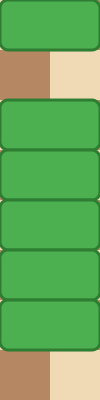
\includegraphics[width=1cm]{2x8.png}
\includegraphics[width=4cm]{3x4_outlined.png}
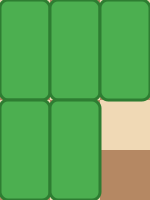
\includegraphics[width=1.5cm]{3x4.png}

\end{document}